\section{Fission Gas Behaviour}

This section examines the behaviour of the two primary gases produced by fission events, Xenon (Xe) and Krypton (Kr), focusing on their impact on design parameters such as the plenum height.

Both Xe and Kr are chemically inert gases with a combined fission yield of approximately 30\% (including contributions from other fast-decay fission products that convert into Xe and Kr within minutes).

Fission events lead to a constant production of fission gas atoms distributed throughout the fuel, resulting in two key phenomena: Fuel Gaseous Swelling and Fission Gas Release (FGR).

\subsection{Fission Gas Release}

Through diffusion, a portion of the fission gas produced in the fuel is released into the plenum. This release "pollutes" the helium initially present in the plenum, reducing its thermal conductivity and increasing the internal pressure of the pin as additional gas moles accumulate within a fixed volume.

These phenomena occur continuously under irradiation and influence the thermo-mechanical behaviour of the fuel pin in a highly non-linear manner. Accurate prediction and control are essential for safe operation.

The problem is addressed using Rate Theory Equations coupled with Cluster Dynamics considerations. The phenomenon is modeled at the grain scale, which serves as the domain for the analysis. The following equations are solved:

\paragraph{Total Gas Production}
The total amount of gas produced is governed by a simple ordinary differential equation:
\begin{equation}
    \frac{dP}{dt} = y \cdot \dot{F}
\end{equation}
where:
\begin{itemize}
    \item $P \, \left(\frac{\text{at}}{\text{m}^3}\right)$: Gas produced.
    \item $y$: Fission yield (combined for Xe and Kr).
    \item $\dot{F}$: Fission rate.
\end{itemize}

\paragraph{Intra-granular Gas Behaviour}
The intra-granular behaviour of fission gases is described by:
\begin{equation}
    \frac{dG_M}{dt} = D_{\text{eff}} \cdot \nabla^2 G_M + y \cdot \dot{F}
\end{equation}
where:
\begin{itemize}
    \item $G_M \, \left(\frac{\text{at}}{\text{m}^3}\right)$: Gas retained by the grain.
    \item $D_{\text{eff}}$: Effective diffusivity, encompassing all relevant phenomena.
\end{itemize}

\subsection{Main Assumptions, Data, and Hypotheses}

\begin{itemize}
    \item \textbf{Domain size}: Grain size $d_g = 10\,\mu \text{m}$.
    \item \textbf{Diffusivity model}: Matzke (1980):
    \begin{equation}
        D_{\text{eff}} \, [\text{m}^2/\text{s}] = D_0 \cdot \exp\left(-\frac{Q}{T}\right)
    \end{equation}
    where $D_0 = 5 \cdot 10^{-8} \, \text{m}^2/\text{s}$, $Q = 40262$, and $T$ is the temperature in Kelvin.
    \item \textbf{Reference temperature}: Average of the three main axial temperatures (first slice, midplane, last slice).
    \item \textbf{Fission yield}: Combined yield for Xe and Kr, $y = 30\%$.
    \item \textbf{Fission rate}:
    \begin{equation}
        \dot{F} = \Sigma_f \cdot \phi_{\text{avg}}
    \end{equation}
    where $\Sigma_f$ is the macroscopic fission cross section and $\phi_{\text{avg}}$ is the average neutron flux.
    \item \textbf{Initial conditions}: $P(0) = 0$, $G_M(0) = 0$.
    \item \textbf{Boundary conditions} (Booth, 1957):
    \begin{itemize}
        \item Surface: Perfect sink, $G_M(a) = 0$.
        \item Center: Symmetry, $\frac{dG_M(0)}{dr} = 0$.
    \end{itemize}
    \item \textbf{Steady-state assumption}: Given the short timescale of the phenomenon, the system is assumed to stabilize quickly. The time derivative is neglected for the steady-state solution.
\end{itemize}

\subsection{Results and Comments}

\subsubsection{Total Gas Produced}

The total amount of gas produced is computed by solving the equation:
\begin{equation}
    \frac{dP}{dt} = Y_f \cdot \dot{F}
\end{equation}
At $t = 360 \, \text{days}$, the total gas produced is:
\[
P(1y) = 1.23 \cdot 10^{27} \, \text{at/m}^3
\]

\begin{figure}[H]
    \centering
    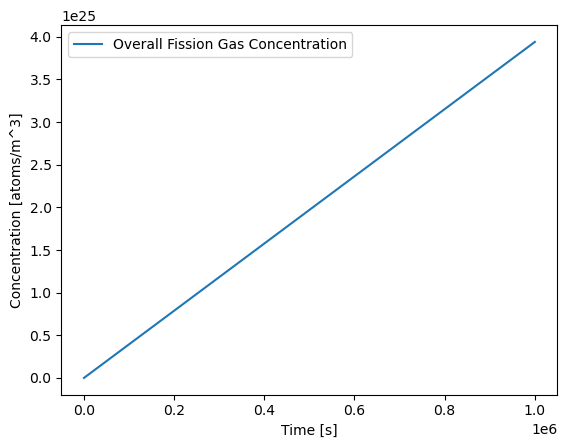
\includegraphics[width=0.8\textwidth]{FGR_1.png}
    \caption{Overall Fission Gas Concentration.}
    \label{fig:FGR_1}
\end{figure}

\subsubsection{Gas Retained by Grain}

The spatial distribution of retained gas, $G_M$, is shown below:
\begin{figure}[H]
    \centering
    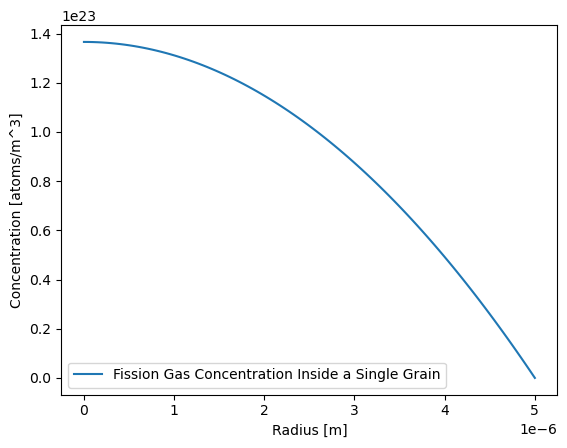
\includegraphics[width=0.8\textwidth]{FGR_2.png}
    \caption{Fission Gas Concentration Inside a Single Grain.}
    \label{fig:FGR_2}
\end{figure}

Integrating this curve across the grain domain and multiplying by the number of grains per pellet and pellets per pin provides the total amount of gas retained in the fuel.

The difference between the total gas produced and the gas retained gives the total Fission Gas Release (FGR).

\begin{table}[H]
    \centering
    \caption{Summary of Computed Parameters and Quantities}
    \begin{tabular}{|c|c|}
        \hline
        \textbf{Parameter} & \textbf{Value} \\
        \hline
        $\Sigma_f$ & 0.027 cm$^{-1}$ \\
        $\phi_{\text{avg}}$ & $4.87 \cdot 10^{15}$ n/cm$^2 \cdot$ s \\
        $\dot{F}$ & $1.31 \cdot 10^{20}$ fissions/m$^3 \cdot$ s \\
        $T_{\text{avg}}$ & 2349.25 K \\
        $D_{\text{eff}}$ & $1.8 \cdot 10^{-15}$ m$^2$/s \\
        $P(1y)$ & $1.23 \cdot 10^{27}$ at/m$^3$ \\
        $G_M(1y)$ & $1.10 \cdot 10^{25}$ at/m$^3$ \\
        FGR & $1.21 \cdot 10^{27}$ at/m$^3$ \\
        \hline
    \end{tabular}
    \label{tab:fgr_summary}
\end{table}

\subsection{Impact on the Design}

The FGR contributes to increased internal pin pressure, which may affect cladding integrity. The maximum allowable internal pressure is set at $5 \, \text{MPa}$. Using the ideal gas law:
\begin{equation}
    p \cdot V = n \cdot R \cdot T
\end{equation}
the effect of different plenum heights on internal pressure is evaluated.

\begin{figure}[H]
    \centering
    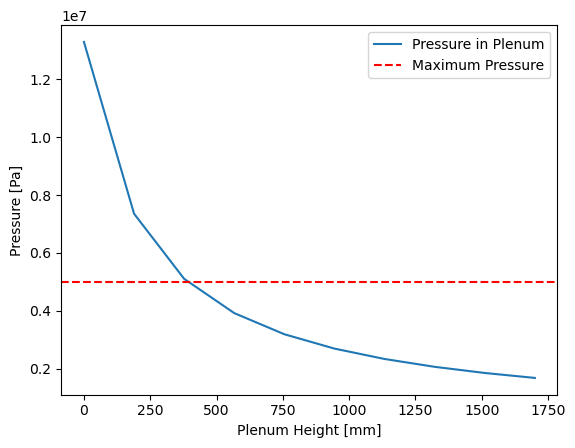
\includegraphics[width=0.9\textwidth]{FGR_3.png}
    \caption{Pressure in Plenum vs. Plenum Height.}
    \label{fig:plenum_pressure}
\end{figure}

Additionally, FGR reduces the thermal conductivity of the gap filling gas, increasing the fuel temperature. This temperature rise enhances FGR, creating a positive feedback loop. Iterative calculations account for this feedback to reach stable temperature and FGR values.
